\documentclass[a4paper, 11pt, final, garamond]{book}
\usepackage{cours-preambule}

\makeatletter
\renewcommand{\@chapapp}{Devoir surveill\'e -- num\'ero}
\makeatother

\begin{document}
\setcounter{chapter}{1}

\def\lspace{25}

\chapter{Commentaires sur le DS \oldno02}

\section{Commentaires généraux}

DS décevant. Les définitions ne sont pas connues, les ponts diviseurs non plus,
les bases sont complètement ignorées. Mathématiquement il y a des sacrilèges et
des crimes innommables, c'est vraiment grave et inquiétant. Il faut vraiment
vous y mettre, utiliser les cahiers d'entraînement, pratiquer pratiquer
pratiquer.

Le vocabulaire de base est parfois, mais gravement, pas maîtrisé. Une
\textbf{tension est aux bornes} d'un dipôle, une \textbf{intensité traverse} un
dipôle.

% \begin{tcb}[bld,cnt,fontupper=\Large](impo){Points clés}
% 	\begin{itemize}
% 		\item Les interrupteurs, ouverts ou fermés, ne sont PAS des résistances~!
% 		\item Interrupteur fermé (fil) $\Ra i \neq 0, u = 0$~;
% 		\item Interrupteur ouvert $\Ra i=0, u \neq 0$~!
% 		\item Condition initiale $\cancel{\Lra}$ en $t=0$, mais en $t$ initial~!
% 	\end{itemize}
% \end{tcb}

\textbf{Les tensions ne sont pas des vecteurs~!!}

\begin{center}
	\fatbox{%
		\large \bfseries
		ARRÊTEZ AVEC LES $\times$ QUI RESSEMBLENT À DES $+$~!!
	}%
\end{center}
Arrêtez avec les $\times$ tout court~! Pour la peine, nouveau malus $-$X.

\begin{center}
	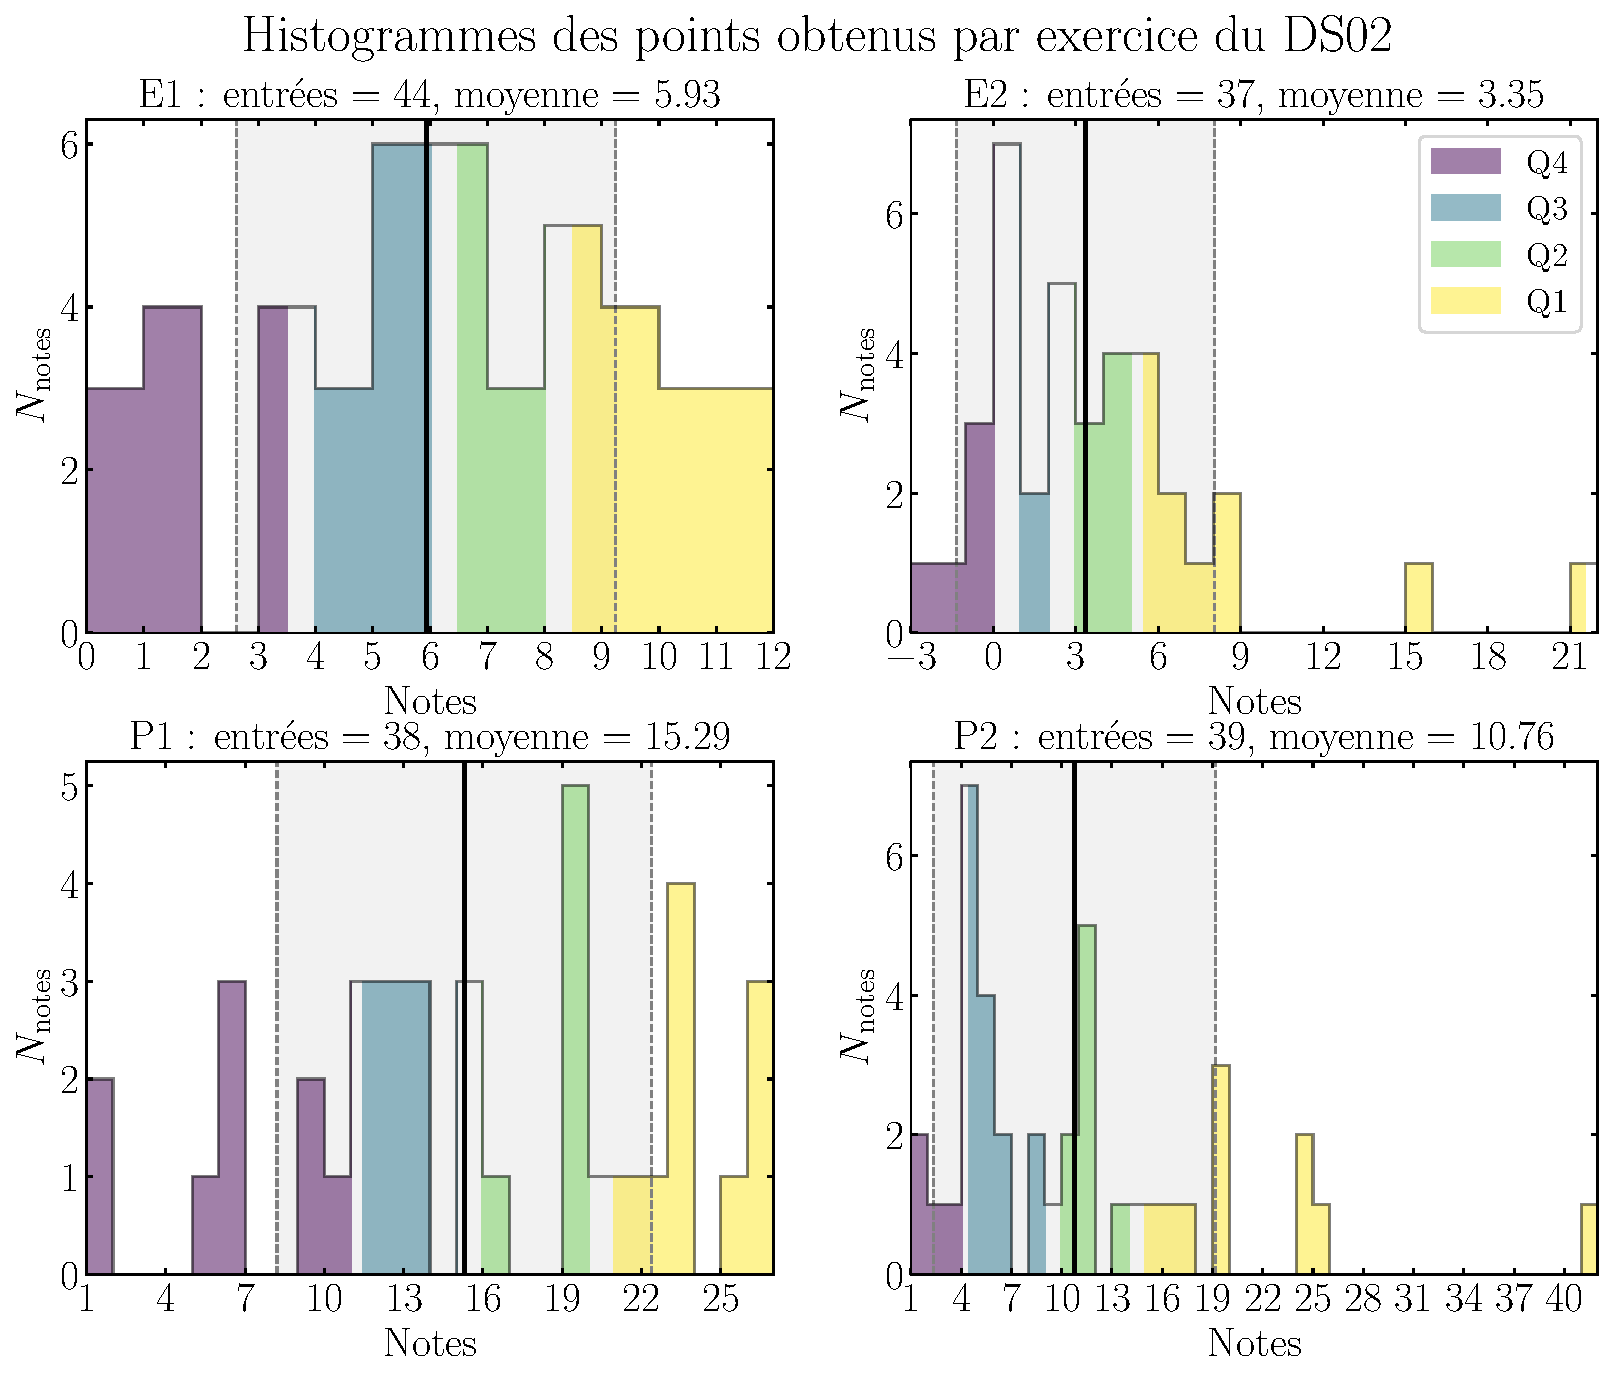
\includegraphics[width=.8\linewidth]{DS02_hist_all.pdf}
\end{center}

\setcounter{section}{0}
\section[24]"E"{Circuit de résistances}

C'est \textbf{intolérable de ne pas refaire de schémas}. Il va falloir vraiment
travailler le fait de faire des schémas tout le temps, toute l'année, pour tout,
pour toujours, à jamais, forever, para siempre, bref, on fait de la
physique-chimie il faut s'y mettre.

\begin{enumerate}[label=\sqenumi]
	\item[n]{5}% Q1
	      Les définitions de série et parallèle ne sont pas maîtrisées. C'est
	      grave.
	\item[n]{4}% Q2
	      Pas trop de problèmes d'inhomogénéité, bravo~! Par contre,
	      \textbf{faites le schéma équivalent}. De même, \textbf{il faut repartir
		      de $1/R\ind{eq} = 1/R_1 + 1/R_2$}.
	      \smallbreak
	      Très dommage pour les réponses $R_{AB} = 2R$. Il faut savoir placer
	      les points sur un schéma et ne pas vont plonger dans une lecture
	      superficielle.
	      \begin{center}
		      \fatbox{%
			      \large \bfseries
			      $\frac{1}{R} + \frac{1}{R} = \frac{1}{2R}$ c'est un CRIME
		      }%
	      \end{center}
	\item[n]{4}% Q3
	      Idem, schémas équivalents.
	\item{}[\fbox{4-5}] % Q4-5
	      Il \textbf{faut} voir les PdT et PdC. Entraînez-vous à les identifier.
	      \textbf{Beaucoup de problèmes de signes} à cause du fléchage. Il faut
	      savoir
	      revenir exactement à la situation du cours~!
	      \smallbreak
	      Vous ne pouvez pas trouvé un $I_k > I\ind{para}$, par définition du
	      \textbf{diviseur} de courant~!
\end{enumerate}

\setcounter{section}{0}
\section[47]"P"{Alimentation d'un train}
\begin{enumerate}[label=\sqenumi]
	\item[n]{3}% Q1
	      Bien. Attention, \textbf{convention $\neq$ réalité}.
	\item[n]{2}% Q2
	      Bien.
	\item[n]{5}% Q3
	      \textbf{Il faut \xul{choisir} la bonne valeur} dans le résultat d'un
	      trinôme~! À la fin, il n'y a bien qu'une seule tension… Énoncé peu clair
	      nonobstant.
	      \smallbreak
	      Arrêtez avec les applications numériques sauvages~! Et toute grandeur
	      physique a une unité, même un discriminant.
	\item[n]{4}% Q4
	      Exercice très peu compris.
	\item[n]{3}% Q5
	      Correct.
	\item[n]{3}% Q6
	      \textbf{Convention générateur} pour la résistance $r_N$, donc loi
	      d'\textsc{Ohm} est opposée~! De toute façon, le générateur ne va pas
	      envoyer plus de tension quand on a plus de courant, la résistance
	      dissipe l'énergie… soyez critiques.
	\item[n]{2}% Q7
	      Il y a unicité de l'intensité dans une branche et de la tension aux bornes
	      d'un dipôle, donc si les deux dipôles sont les mêmes ils ont forcément $u_N
		      = u_{th}$ et $i_N = i_{th}$~!
	\item[n]{4}% Q8
	      TB.
	\item[n]{6}% Q9
	      Revenez à la définition des générateurs en les séparant~: ici, en
	      séparent les générateur de \textsc{Thévenin} de gauche, $R_{c_1}$ et
	      $R_{r_1}$ sont en série~!
	\item{}[\fbox{10-13}] % Q10
	      Non faites.
\end{enumerate}

\section[66]"P"{Étude d'une lampe de secours rechargeable}
\begin{enumerate}[label=\sqenumi]
	\item[n]{10}% Q1
	      \vspace{-22pt}
	      \begin{itemize}
		      \item \textbf{RCT convention générateur}~!! Ça doit vous
		            \textbf{choquer} d'avoir un signe $-$ devant l'ordre 0. Ça nous
		            donnerait une exponentielle qui diverge en $t \to \infty$~!
		      \item Par continuité de la tension \textbf{aux bornes de $C$}~!
		      \item Des temps négatifs… malus \circled{$-\f$}.
		      \item Respectez les notations de l'énoncé. Ici, $u_C(0) = U_0 \neq E$.
		      \item Arrêtez (encore) avec les applications numériques sauvages et le
		            mélange littéral-numérique
	      \end{itemize}
	\item[n]{3}% Q2
	      \textbf{Pas besoin de démontrer $t_{99} \approx 5\tau$}. Attention aux
	      applications numériques mal faites et le mélange littéral-numérique
	      (\textbf{encore}).
	      \smallbreak
	      Vous vous rendez compte que vous essayez de résoudre $\exr^{x} = 0$~?
	      Mathématiquement, une exponentielle ne s'annule jamais~! On définit une
	      décharge à partir d'une certaine valeur.
	\item[n]{4}% Q3
	      Majoritairement mal faite. Il faut vous créer une intuition sur les
	      résistances et leur fonctionnement limite (fil et interrupteur ouvert).
	\item[n]{14}% Q4
	      Très peu correctement traitée.
	\item[n]{6}% Q5
	      La \textbf{résistance est remplacée} par la diode.
	\item[n]{8}% Q6
	      Assez moyen. Pas besoin de redémontrer la forme de la solution homogène
	      quand vous l'avez déjà fait question 1.
	\item[n]{5}% Q7
	      On l'a eu. $u_C = Ri$. C'est dur. Pour rappel, $u = Ri$ ne vaut
	      \textbf{que pour les résistances}~!!
	\item[n]{6}% Q8
	      Tant de chatons morts…
	      \smallbreak
	      \textbf{Conditions initiales sur solution générale totale, pas sur
		      homogène}~!!
	\item{}[\fbox{9-10}] % Q9
	      Non faite.
\end{enumerate}

\section[71]"P"{Guirlandes électriques}
Attention à l'énoncé~: «~\textbf{Les expressions demandées ne feront intervenir
	que $E$, $r$ et $R$}~»~!
\begin{enumerate}[label=\sqenumi]
	\item[n]{2}% Q1
	      Bien.
	\item[n]{6}% Q2
	      Littéralement premier exercice du premier TD d'électricité.
	\item[n]{5}% Q3
	      Faire le schéma équivalent.
	\item[n]{3}% Q4
	      Très mal faite… attention aux notations, soyez précis-es.
	\item[n]{2}% Q5
	      Correct avec des magouilles.
	\item[n]{3}% Q6
	      Correct.
	\item[n]{3}% Q7
	      Bien. Détaillez le pourquoi du comment.
	\item[n]{2}% Q8
	      RAS, globalement mal fait.
	\item[n]{3}% Q9
	      Correct, mais il faut bien définir quel $i$ on obtient. En l'occurrence,
	      c'est $i_o$ de la question 2.
	\item[n]{5}% Q10
	      $i_2$ pas continue, puisque pas de bobine~! Très mal géré.
	\item{}[\fbox{11-18}]% Q11
	      RAS.
\end{enumerate}

\end{document}
